\documentclass[12pt]{article}
\usepackage{geometry}                % See geometry.pdf to learn the layout options. There are lots.
\geometry{letterpaper}                   % ... or a4paper or a5paper or ... 
%\geometry{landscape}                % Activate for for rotated page geometry
\usepackage[parfill]{parskip}    % Activate to begin paragraphs with an empty line rather than an indent
\usepackage{daves,fancyhdr,natbib,graphicx,dcolumn,amsmath,lastpage,url}
\usepackage{amsmath,amssymb,epstopdf,longtable}
\usepackage{paralist}  % need to modify standard enumerate blocks
\usepackage[final]{pdfpages}
\DeclareGraphicsRule{.tif}{png}{.png}{`convert #1 `dirname #1`/`basename #1 .tif`.png}
\pagestyle{fancy}
\lhead{CE 3354 -- Engineering Hydrology}
\rhead{FALL 2025}
\lfoot{ES2}
\cfoot{}
\rfoot{Page \thepage\ of \pageref{LastPage}}
\renewcommand\headrulewidth{0pt}



\begin{document}
\begin{center}
{\textbf{{ CE 3354 Engineering Hydrology} \\ {Exercise Set 2}}}
\end{center}

\section*{\small{Exercises}}
\begin{enumerate}
\item A raingage is located in a 2.5 acre impervious watershed with non initial abstraction.  The gage records a catch of 1.0 inches of precipitation in one hour.  The maximum intensity was 2.4 inches per hour for 10 minutes.  Assume that 10 minutes is the characteristic time for which all parts of the watershed can contribute runoff to a discharge point.

Determine:
    \begin{enumerate}[a)]
        \item Volume of rainfall in cubic feet for the watershed. 
        \item Maximum (peak) discharge rate for the watershed.
    \end{enumerate}

\clearpage

\item Consider the rainfall data in Table \ref{tab:SomewhereUSARain}

\begin{table}[h!]
\centering
\caption{Somewhere USA Precipitation Data}
\begin{tabular}{p{2.0in}p{2.0in}} % Column formatting, @{} suppresses leading/trailing space
~&~\\
Time (minutes) & Cumulative Depth (inches\\
\hline
\hline
0.00 & 0.00 \\
30.0 & 0.04 \\
60.0 & 0.38 \\
90.0 & 1.07 \\
120. & 1.44 \\
150. & 1.62 \\
180. & 1.70 \\
\hline
\end{tabular}
\label{tab:SomewhereUSARain}
\end{table}

Determine:
    \begin{enumerate}[a)]
        \item A depth (cumulative inches) hyetograph in 30 minute intervals (plot). 
        \item An intensity (inches/hour) hyetograph in 30 minute intervals (plot).
    \end{enumerate}

\clearpage

\item The intersection of US 408 and US 417 in Orange County, Florida at 28°32'51.2"N 81°15'28.5"W is the approximate centroid of that county. Using NOAA Atlas 14 (use the online PFDS tool)

Determine:
    \begin{enumerate}[a)]
        \item The 1-hr rainfall depth for a 100-yr Annual Recurrance Interval (ARI). 
        \item The 1-hr average rainfall intensity for a 100-yr Annual Recurrance Interval (ARI). 
        \item The 6-hr rainfall depth for a 100-yr Annual Recurrance Interval (ARI). 
        \item The 1-hr average rainfall intensity for a 100-yr Annual Recurrance Interval (ARI). 
    \end{enumerate}

\clearpage

\item 55 mm of rain is recorded for a 6-hour storm by a raingage for a 10 km$^2$ watershed.  The runoff from the storm indicates that only 45 mm of rain fell on the entire area.  

    \begin{enumerate}[a)]
        \item The areal reduction factor  (ARF). 
        \item Compare the result to Central Texas areal reduction factors 
    \end{enumerate}

\clearpage

\begin{table}[h!]
\centering
\caption{Somewhere Else USA Precipitation Data -- End of Interval Catch}
\begin{tabular}{p{2.0in}p{2.0in}} % Column formatting, @{} suppresses leading/trailing space
~&~\\
Time (hours) & Cumulative Depth (inches\\
\hline
\hline
0.00 & 0.00 \\
0.25 & 0.10 \\
0.50 & 0.21 \\
0.75 & 0.33 \\
1.00 & 0.48 \\
1.25 & 0.64 \\
1.50 & 0.81 \\
1.75 & 1.08 \\
2.00 & 1.38 \\
2.25 & 2.46 \\
2.50 & 3.60 \\
2.75 & 3.90 \\
3.00 & 4.20 \\
3.25 & 4.44 \\
3.50 & 4.68 \\
3.75 & 4.86 \\
4.00 & 5.01 \\
4.25 & 5.16 \\
4.50 & 5.28 \\
4.75 & 5.40 \\
5.00 & 5.52 \\
5.25 & 5.64 \\
5.50 & 5.76 \\
5.75 & 5.88 \\
6.00 & 6.00 \\
\hline
\end{tabular}
\label{tab:SomewhereElseUSARain}
\end{table}

Determine:
    \begin{enumerate}[a)]
        \item The average rainfall intensity (inches/hour) from hour 3:00 to hour 4:00. 
        \item The average rainfall intensity (inches/hour) for the first half of the storm. 
        \item The maximum rainfall intensity (inches/hour) in any one hour.  
        \item The maximum rainfall intensity (inches/hour) in any 15-minute interval. 
        \item The average rainfall intensity (inches/hour) for the last half hour of the storm.   
    \end{enumerate}

\clearpage

\item Using the NRCS Type III rainfall distribution

Determine:
    \begin{enumerate}[a)]
        \item The cumulative rainfall depth (inches) for half-hour increments for a 10 inch total depth, 24-hour storm.
        \item The rainfall intensity (inches/hour) for each half-hour increment of the storm. 
        \item The maximum rainfall intensity (inches/hour) in any 30-minute interval.  
    \end{enumerate}

\clearpage

\item The map excerpt in Figure \ref{fig:usgsmap}, shows a stream gage labeled as U.S.G.S. no. 1.  Various rain gages are shown as rectangles surrounding the catch for the gage for some time interval.  

\begin{figure}[h!] %  figure placement: here, top, bottom, or page
   \centering
   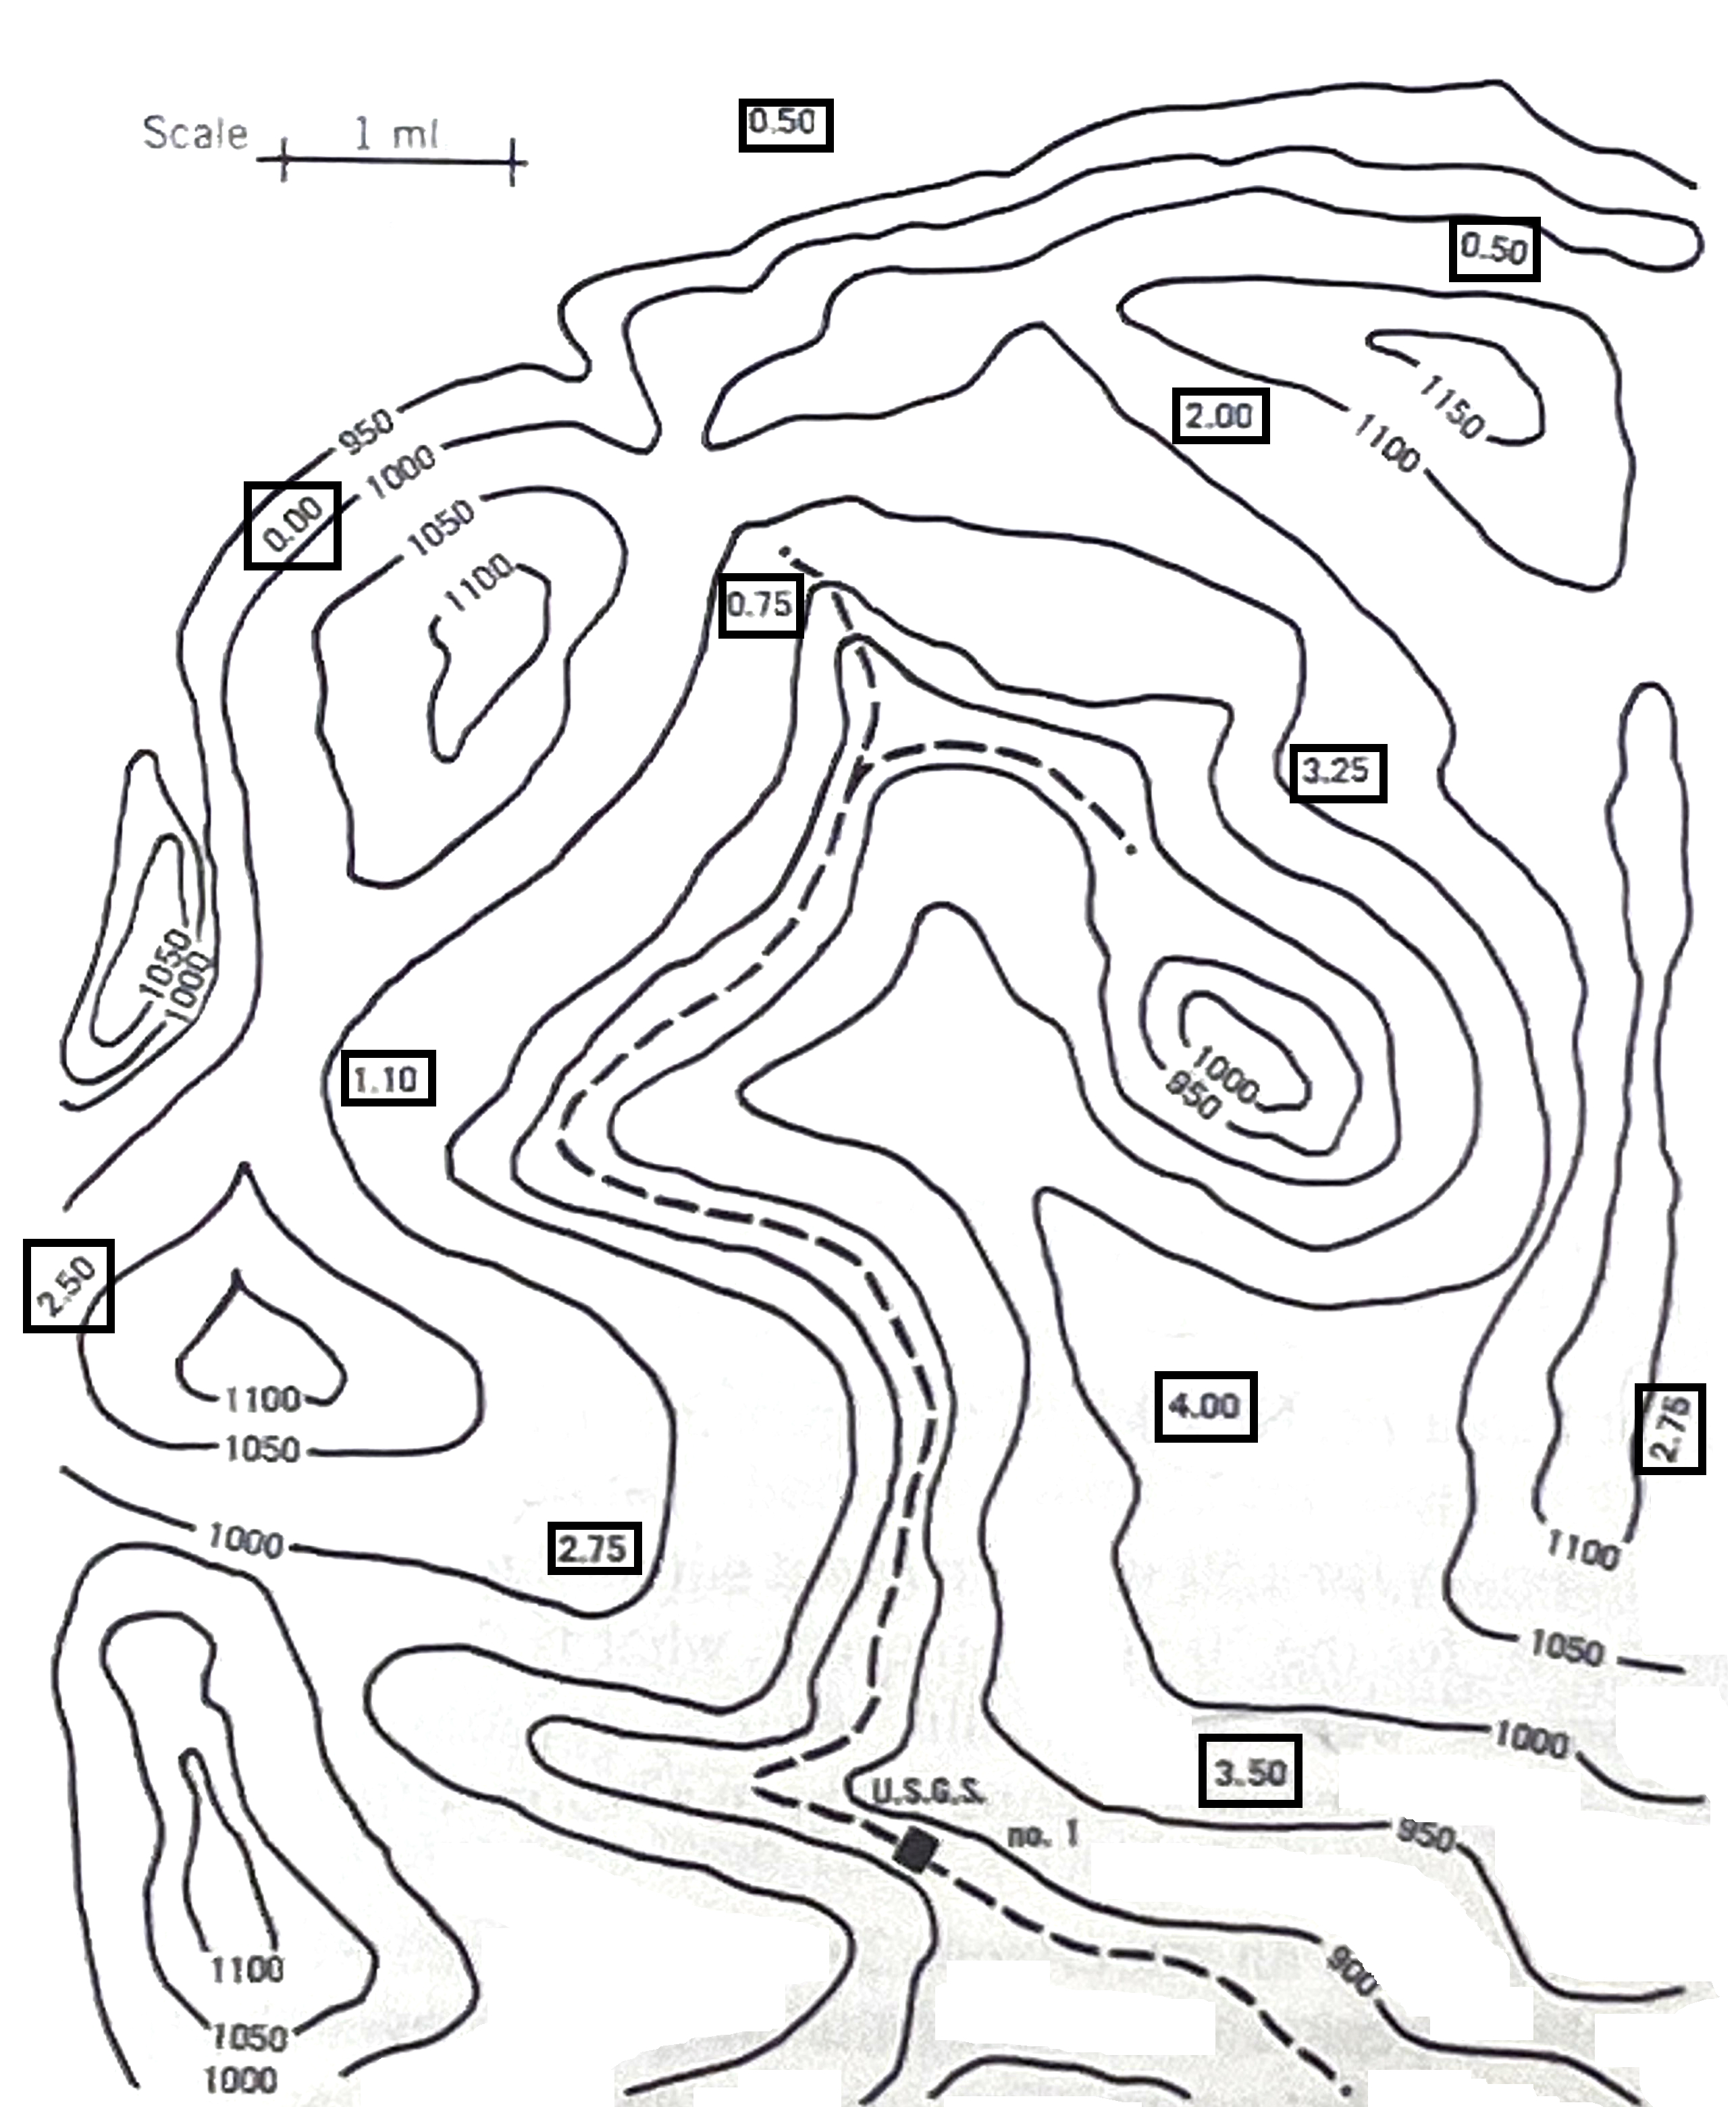
\includegraphics[height=5in]{Map.jpg} 
   \caption{U.S.G.S. No. 1 Area Map}
   \label{fig:usgsmap}
\end{figure}

Determine:
    \begin{enumerate}[a)]
        \item The drainage area boundary using watershed delineation principles.
        \item The drainage area in square miles. 
        \item The average precipitation over the area by arithmetic mean. 
        \item The average precipitation over the area by Thiessen polygon method. 
        \item The average precipitation over the area by Isoheytal method
    \end{enumerate}


\clearpage

\item Table \ref{tab:SomewhereUSARainIDF} is intensity duration data for Somewhere USA.

\begin{table}[h!]
\centering
\caption{Somewhere USA Intensity-Duration}
\begin{tabular}{p{2.0in}p{2.0in}} % Column formatting, @{} suppresses leading/trailing space
~&~\\
Duration (minutes) & Intensity (inches/hour) \\
\hline
\hline
10.0 & 4.00 \\
15.0 & 3.20 \\
20.0 & 2.70 \\
30.0 & 1.90 \\
60.0 & 1.20 \\
120. & 0.80 \\
180. & 0.60 \\
\hline
\end{tabular}
\label{tab:SomewhereUSARainIDF}
\end{table}

Determine:
    \begin{enumerate}[a)]
        \item Plot the intensity duration on the plot type that produces a straight line.
        \item An equation (model) of the "best" straight line for these values. 
    \end{enumerate}

\clearpage

\item Table \ref{tab:Baltimore} is a measured 1-hour hyetograph for Baltimore, Maryland.

\begin{table}[h!]
\centering
\caption{Baltimore, Maryland Rainfall Data}
\begin{tabular}{p{2.0in}p{2.0in}} % Column formatting, @{} suppresses leading/trailing space
~&~\\
Time (minutes) & Intensity (cm/hour) \\
\hline
\hline
0.00 - 10.0 & 2.00 \\
10.0 - 20.0 & 6.00 \\
20.0 - 30.0 & 12.00 \\
30.0 - 40.0 & 8.00 \\
40.0 - 50.0 & 6.00 \\
50.0 - 60.0 & 3.00 \\
\hline
\end{tabular}
\label{tab:Baltimore}
\end{table}

Determine:
    \begin{enumerate}[a)]
        \item The average intensity in cm/hr.
        \item The net volume of rainfall in m$^3$ and liters if the watershed is 4,000 m$^2$
        \item An approximate Annual Recurrance Interval (ARI) for the measured event, using NOAA Atlas 14. 
    \end{enumerate}

    
\end{enumerate}


\end{document}  